Det er mange som søker på studiet basert på navnet, uten egentlig å vite hva man ender opp med å bli. Eller, man blir jo sivilingeniør (selv om man kanskje ikke helt vet hva de gjør med mindre foreldrene dine er sivilingeniører). Uansett, la meg starte med en liten intro.

\begin{remark}
    \textbf{FUN FACT} Vi i Norge får utdanningen gratis, men det gjelder ikke alle. For studenter utenfor EU/EØS så må de betale, men hvor mye da? Prislappen på siving. ligger på 250 000 kr i året! \cite{ntnu_studieavgift}
\end{remark}


\section{Historie}

Studiet MTKJ har ikke eksistert siden tidenes morgen, men har røtter fra teknisk kjemi ved NTH. En interessant anekdote er at NTH ved åpningen rundt 1910 kun hadde én kvinnelig student, og hun studerte selvfølgelig kjemi \cite{Kjemi1910}. Det ryktes at hun ble mobbet av alle de mannlige studentene.

Noen lurer på hvorfor det heter \textit{sivilingeniør}, og det stammer fra behovet for å skille mellom ingeniører utdannet i Forsvaret og sivile ingeniører utdannet ved høyskoler. Ordet sivilingeniør brukes mye i Norden, men det må IKKE forveksles med \textit{civil engineer}, som betyr byggingeniør på engelsk. Det finnes derfor ingen direkte engelsk variant av sivilingeniør; det nærmeste man kommer er \textit{engineer} eller \textit{Master of Science}.

Dagens MTKJ-program spenner over fire institutter, men har tidligere dekket hele elleve institutter! Det er så mye historie om kjemi ved NTH at noen har skrevet en bok om det, \textit{Kjemi ved NTNU gjennom 100 år}. Kanskje jeg leser den etter endt studie \cite{Kjemi100}.

\begin{table}[H]
    \centering
    \begin{minipage}[t]{.8\linewidth}
        \centering
        \color{gray}
        %\rule{\linewidth}{1pt}
        \ytl{1760}{Det Kongelige Norske Videnskabers Selskab blir stifta}
        \ytl{1910}{NTH blir opprettet}
        \ytl{1922}{Noregs lærarhøgskule (seinare AVH) blir opprettet}
        \ytl{1968}{Universitetet i Trondheim (UNIT) opprettes av å sammenslå NTH, AVH og Vitenskapsmuseet}
        \ytl{1996}{NTNU blir opprettet ved å slå sammen UNIT, Det medisinske fakultet (DMF), Kunstakademiet i Trondheim og Musikkonservatoriet.}
        \ytl{2016}{NTNU fusjoneres med Høgskolen i Gjøvik, Høgskolen i Sør-Trøndelag (HiST) og Høgskolen i Ålesund}
        \bigskip
        %\rule{\linewidth}{1pt}
    \end{minipage}
\end{table}

Fra tidslinjen ser vi hvordan dagens NTNU består av mange mindre organisasjoner som over årene har blitt slått sammen. Her kan vi se på opprinnelsen til de ulike studieprogrammene ved dagens NTNU og hvorfor mange studier ligner, selv om de i realiteten er ganske forskjellige. NTH inneholdt alle de eldste sivilingeniørprogrammene, og nyere programmer har blitt lagt til over årene. AVH inneholdt humanistiske fag, biologi, kjemi, fysikk, matematikk, psykologi og informatikk, som danner grunnlaget for mange bachelorprogrammer. Når det gjelder bacheloringeniørprogrammene, stammer de fra fusjonen i 2016 og kommer fra HiST, også kjent som Kalvskinnet. Handelshøyskolen stammer også fra HiST.

\section{Hva er spesialisering og hovedprofil?}

Det finnes mange ukjente ord når man starter på Gløshaugen. Man skulle tro at spesialisering og hovedprofil var det samme, men neida, de er to helt forskjellige ting. La oss derfor først introdusere spesialisering. Her på MTKJ finnes det fire alternativer som heretter vil forkortes til bio, kjemi (anvendt/organisk), prosess og mattek. En oversikt over disse spesialiseringene er vist i Figur \ref{fig:Spesialisering1}.


\begin{figure}[H]
    \centering
    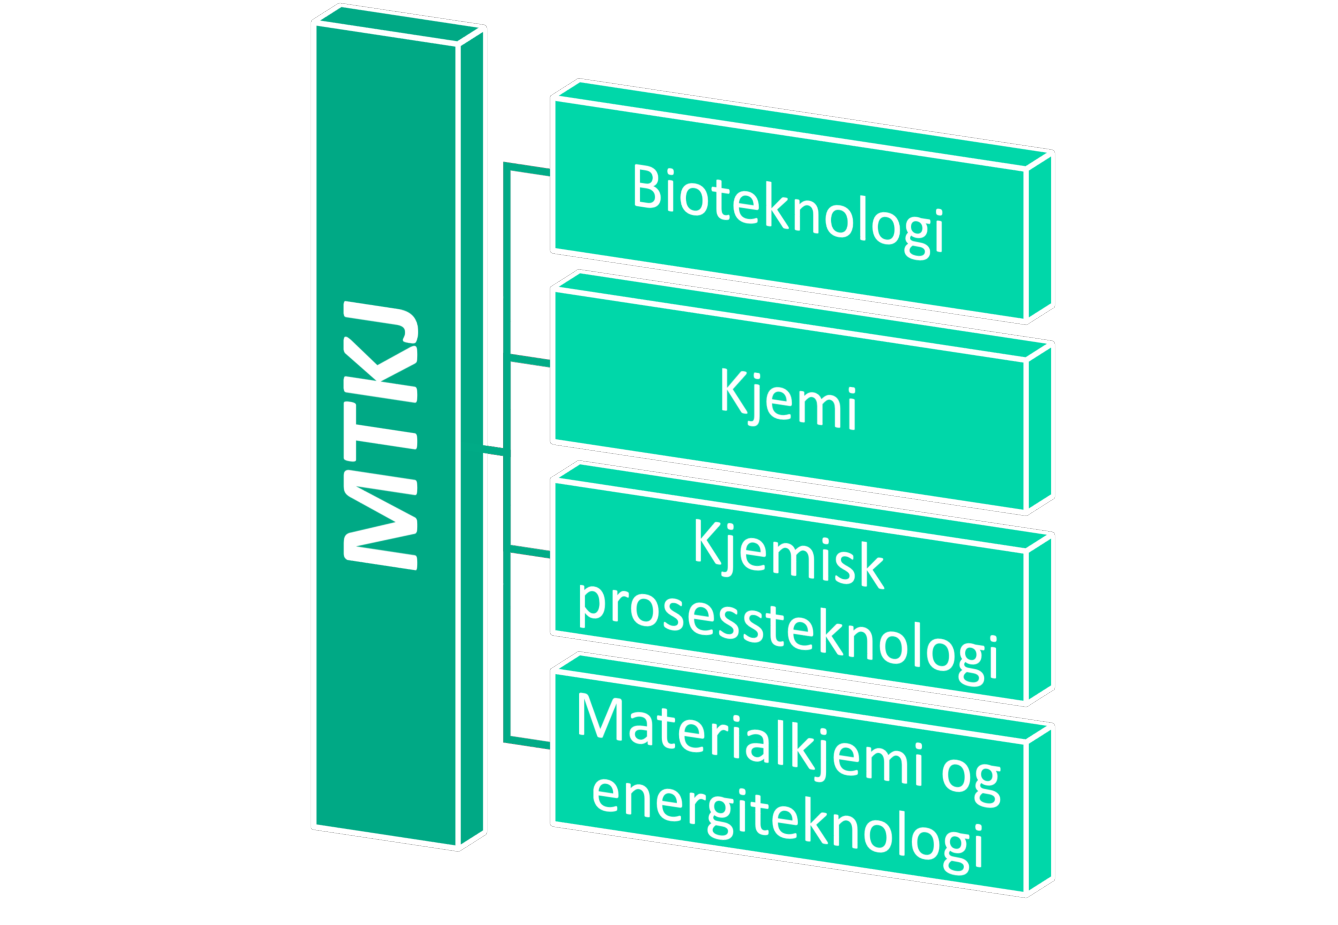
\includegraphics[width=0.8\textwidth]{images/Retningsvalg.pdf}
    \caption{De fire spesialiseringene man kan velge mellom}
    \label{fig:Spesialisering1}
\end{figure}

Valget av spesialisering må tas i løpet av høsten i 3. klasse. Tidligere valgte man spesialisering våren i 2. klasse, men dette ble forskjøvet med et semester fra og med kullet med oppstart i 2019. Det er heller ingen tilfeldighet at hver av spesialiseringene er knyttet til et eget institutt ved Fakultet for Naturvitenskap (NV). Man kan ofte høre prosessfolka snakke om IKP (Institutt for kjemisk prosessteknologi) eller mattek snakke om IMA (Institutt for materialteknologi).

Men hva i all verden er en \textit{hovedprofil}? Det er rett og slett det som kommer etter at man har valgt spesialisering. Dette valget skjer gjerne på et senere tidspunkt, i 4. eller 5. klasse. Det finnes unntak, som for eksempel i retningen \textit{kjemi}, hvor man allerede ved valg av spesialisering også velger hovedprofil (det som HP står for). En oversikt over de ulike hovedprofilene er vist i Figur \ref{fig:Spesialisering-Hovedprofiler}. Det er verdt å merke seg at disse hovedprofilene heller ikke eksisterer ved en tilfeldighet, men reflekterer de ulike forskningsgruppene innad i instituttet. Hvert institutt består ofte av fire forskningsgrupper som hver reflekterer deres fokusområder. Ved IKP finnes det eksempelvis en gruppe innen katalyse, men ikke biomedisin. 

\begin{figure}[H]
    \centering
    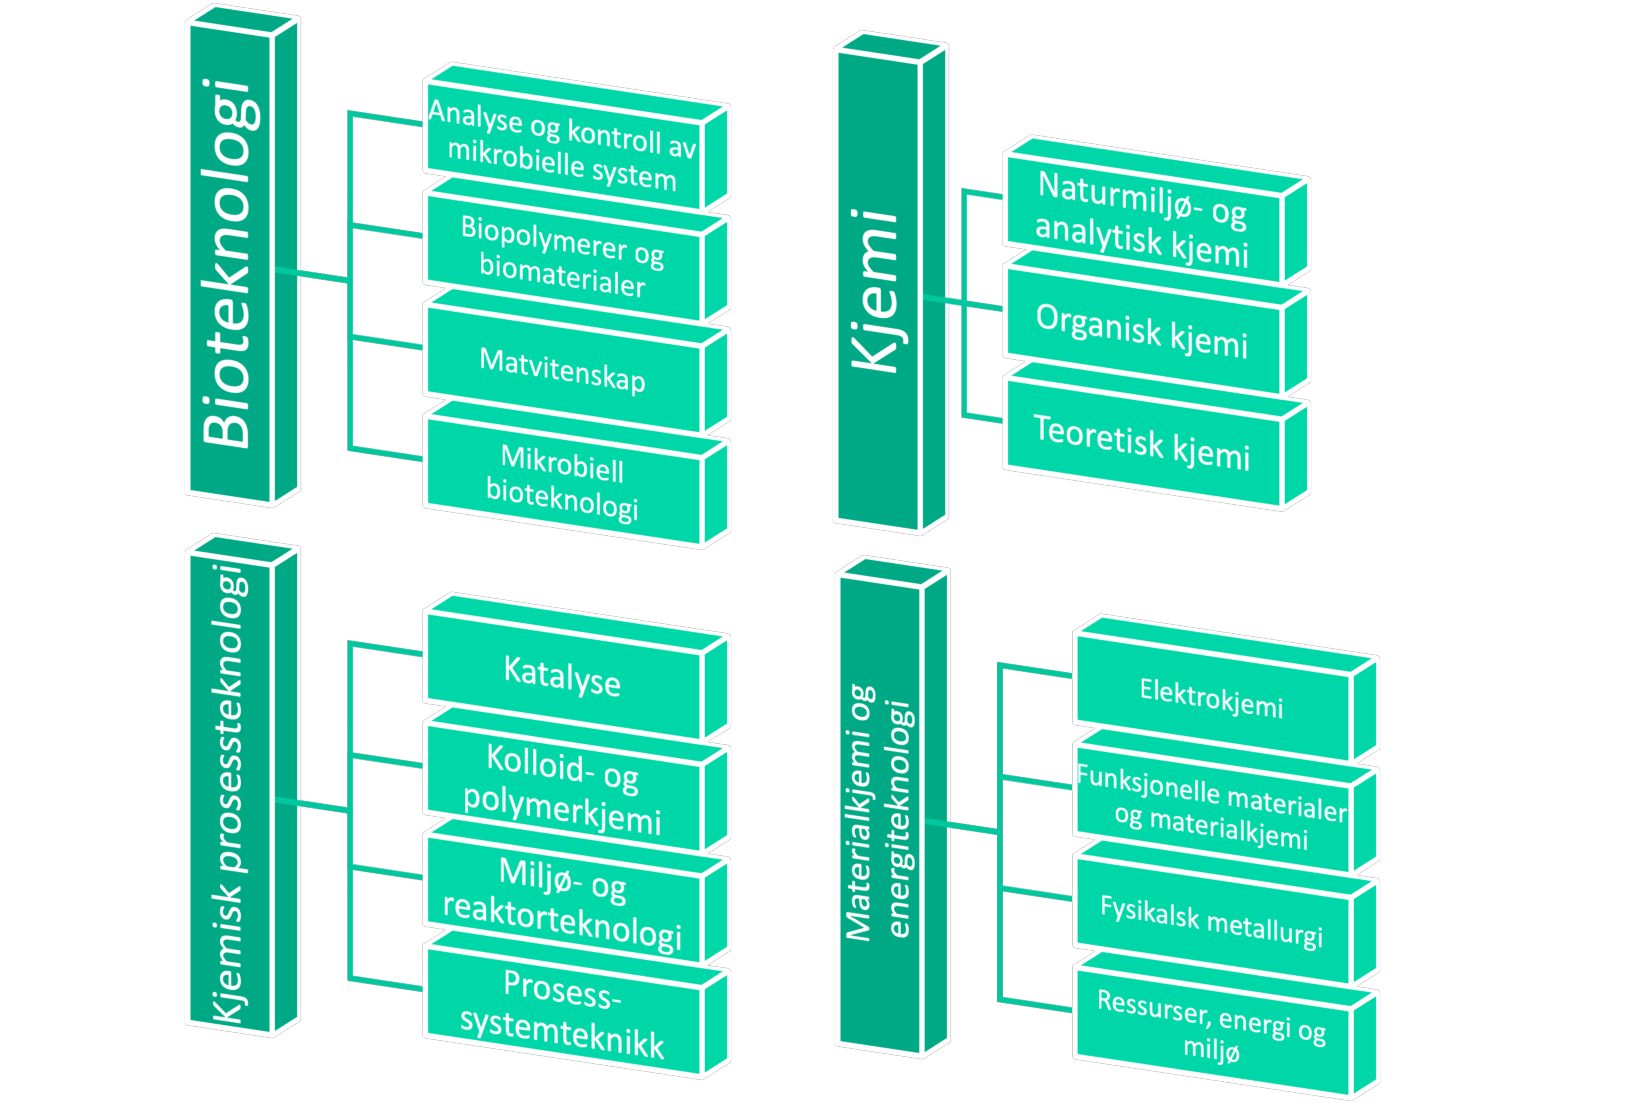
\includegraphics[width=0.9\textwidth]{images/Spesialisering-Retninger.pdf}
    \caption{Oversikt over de mange hovedprofilene man kan velge mellom.}
    \label{fig:Spesialisering-Hovedprofiler}
\end{figure}


\begin{figure}[H]
    \centering
    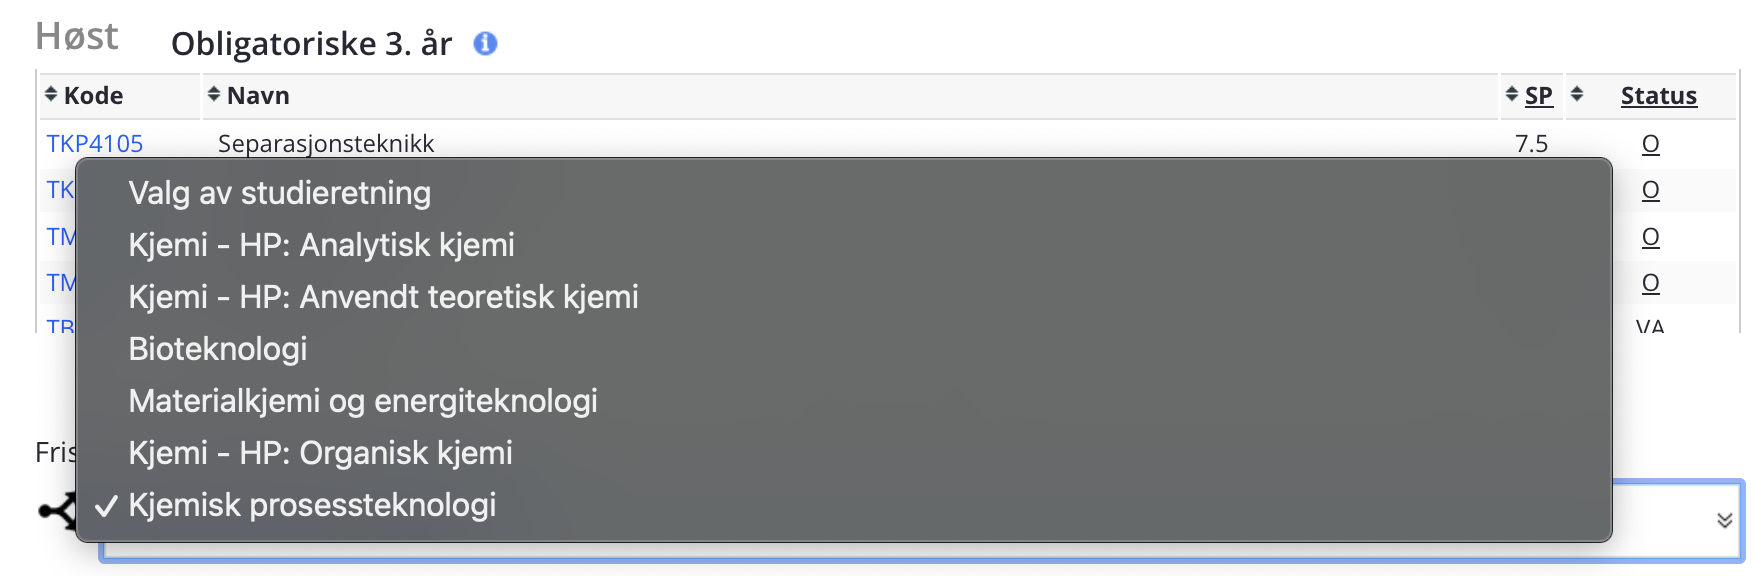
\includegraphics[width=1\textwidth]{images/spesialisering.png}
    \caption{Skjermbilde fra NTNU, dette burde være kjent ;)}
    \label{fig:Spesialisering-Screenshot}
\end{figure}


\section{Hvilken spesialisering bør jeg velge?}

Aha, dette spørsmålet har blitt stilt siden tidenes morgen. Det er et ganske ladd tema som jeg helst unngår å uttale meg om for å unngå heksejakt. Det jeg derimot kan anbefale, er å kikke gjennom listen med ulike ressurser:

\begin{enumerate}
    \item Snakk med en eldre chemiker (åpenbart)
    \item Dra på \textit{Livet etter Kjemi}
    \item \href{https://www.ntnu.no/studier/mtkj/studiets-oppbygning}{MTKJ-siden}
    \item Dra på spesialiseringsmøtene som blir avholdt før valgene
\end{enumerate}

Det er ikke alltid lett å vite hvilken spesialisering man skal velge, men hvis du er nysgjerrig, har jeg samlet en oversikt over spesialiseringene fra 2017-kullet (de som fullførte i 2022) til 2020-kullet (de som fullfører i 2025) i Figur \ref{fig:Spesialisering-Stolpe}.

\begin{figure}[!h]
    \centering
    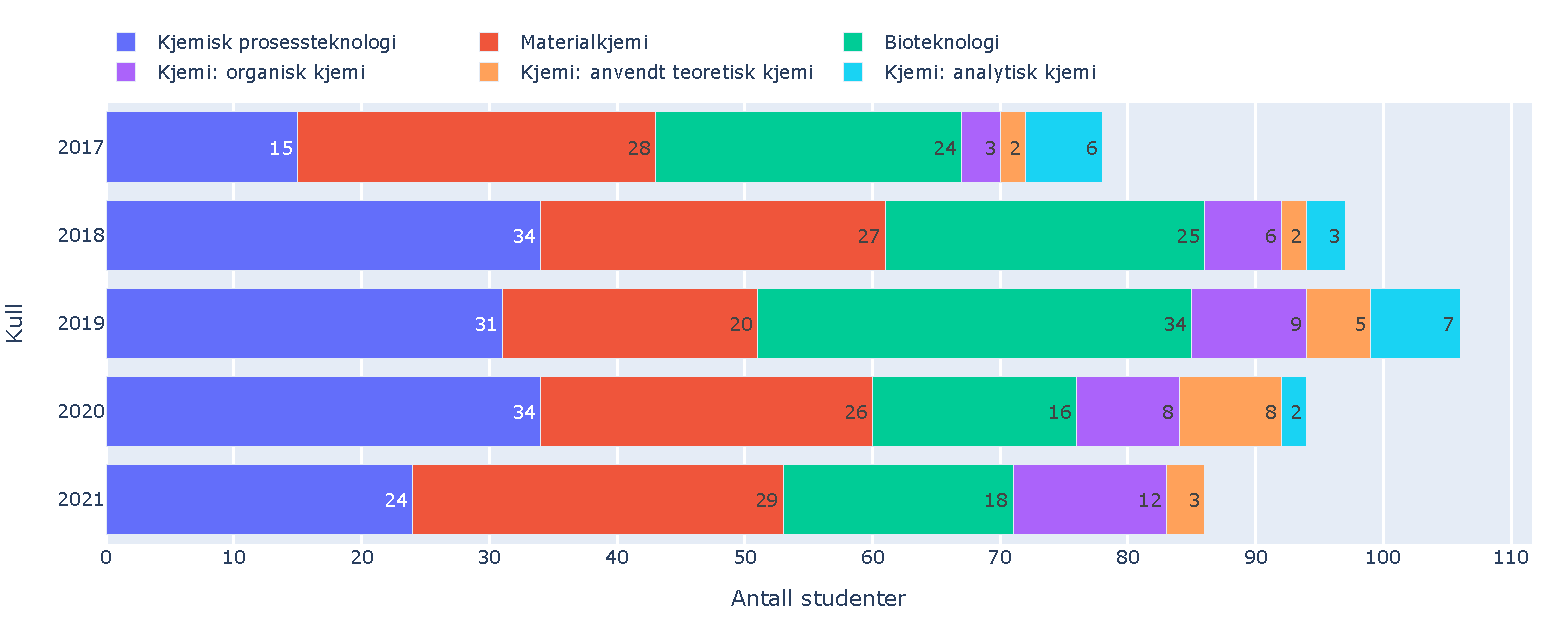
\includegraphics[width=1.1\textwidth]{images/Spesialisering_Stolpe.pdf}
    \caption{Fordeling av spesialisering fra 2017 til 2020-kullet, basert på startår\cite{Hege}}
    \label{fig:Spesialisering-Stolpe}
\end{figure}

Mange lurer spesifikt på jobbmuligheter og hvilke retninger som gir størst sjanse for å få jobb. Hvis du ser på Norges største industrier, er oljebransjen den mest kjente. Det er derfor svært mange muligheter om du jobber direkte i oljeselskaper eller i selskaper som på en eller annen måte har noe med olje å gjøre. I Norge er det også stor produksjon av metaller, typisk aluminium og silisium. Mye av fundamentet bak disse store industriene er kjemisk prosessteknologi og materialteknologi. Derfor er det enklest å få jobb innen disse retningene. Man kan argumentere for at bioteknologi er relevant for fiskeindustrien, men antall sysselsatte der er ikke i nærheten av olje- og metallindustrien. Når det gjelder organisk kjemi, kan man ende opp med arbeid overalt hvor det finnes laboratoriearbeid, men det avhenger igjen av hvor relevant jobben skal være – organisk syntese eller en laborant? Anvendt teoretisk kjemi minner mye om FysMat, og karriereveiene fører ofte til PhD eller konsulentjobb. 


\section{Hvordan ligner MTKJ på de andre studiene ved NTNU?}

Man vil merke at mange studier ved NTNU har flere fellestrekk, og at det til tider bare er en stor grøt med fag og fagfelt. Det kan være lurt å vite hvordan MTKJ ligner på de andre studiene på Gløs, slik at man eventuelt kan bruke dette til å lene seg mot en retning man interesserer seg for, eller finne enkelte fag du får lyst til å ta i løpet av studiet. Her går jeg gjennom alle siving-studiene på Gløs samt noen ekstra studier. 

\begin{table}[H]
    \centering
    \begin{tabular}{p{3cm}p{10cm}}
        \toprule
        Fagfelt & Fellesnevnere \\
        \midrule
        Bygg- og miljøteknikk & Ved å velge mattek kan man ende opp med å arbeide med betong og ulike byggmaterialer. Prosess kan rettes mot vann og avløp. Det er også mulig å bevege seg mot arktisk teknologi ved å velge organisk kjemi. \\
        
        Datateknologi & Vi har tross alt \textit{Informasjonteknologi, grunnkurs}, og noen velger å ta \textit{Prosedyre- og objektorientert programmering (C++)} senere. Den mest populære retningen er kunstig intelligens, hvor mange innen prosess skriver om maskinlæring. I forbindelse med dette kan fag som \textit{Kjemometri}, \textit{Multivariat dataanalyse og maskinlæring} og \textit{Statistisk læring} være nyttige. Man kan derfor lett skrive om maskinlæring uten å være datastudent, slik undertegnede gjør :) \\
        
        Elektronisk systemdesign og innovasjon & Det nærmeste vi kommer er signalbehandling innen prosess. Ellers har vi lite med kretser å gjøre. \\
        
        Energi og miljø & Her er det mye overlapp med en av spesialiseringene til EMIL-studentene. Deres spesialisering \textit{Energi- og prosessteknikk} har mange fellestrekk med prosess, og mange tar derfor \textit{Energiutnyttelse og prosessintegrasjon i industrielle anlegg}. Det skal sies at EMIL-prosess og MTKJ-prosess konkurrerer om de samme jobbene da begge faller under "prosessteknikk". \\
        
        Fysikk og matematikk & Vår kjære FysMat, her er det naturlig mange likheter. Liker du kvantekjemi eller termodynamikk, nærmer du deg spesialiseringen \textit{Teknisk fysikk}. Liker du modellering, optimalisering og statistikk, og velger disse mattetunge retningene i anvendt kjemi, mattek eller prosess, nærmer du deg \textit{Industriell matematikk}. Deres \textit{Biofysikk og medisinsk teknologi} kan minne om en bioretning på matte-steroider. Industrien ansetter også FysMat-studenter, men de fleste jobber heller i forskning eller som konsulenter. \\
        
        Georessurser og geoteknologi & Det nye navnet på sivilingeniørstudiet \textit{Petroleumsfag}, som minner mye om visse retninger innen prosess. Det er ingen hemmelighet at mange fra MTKJ, spesielt prosess, får jobb innen olje og gass. De har også fag som \textit{Prosessteknikk} og \textit{Separasjonsteknikk} som en del av fagplanen. \\
        \bottomrule
    \end{tabular}
    \caption{Hvordan MTKJ ligner på andre studier DEL 1}
    \label{tab:AndreStudierDel1}
\end{table}

\newpage

\begin{table}[H]
    \centering
    \begin{tabular}{p{3cm}p{10cm}}
        \toprule
        Fagfelt & Fellesnevnere \\
        \midrule
        Industriell design & Strengt tatt ikke et sivilingeniørstudie lenger, men om du har interesse for design og farger, kan \textit{Visuell formidling} være interessant. \\
        
        Industriell økonomi og teknologiledelse & Indøk har sine teknologiretninger som er de samme som mange av de nevnte studiene på denne listen, så det tekniske sier seg selv. Men om du er interessert i økonomi og ledelse utover det som blir gjennomgått i \textit{Teknologiledelse}, kan du ta \textit{Finans for teknisk-naturvitenskapelige studenter} eller ta et år ekstra på \textit{Samfunnsøkonomi – bachelor} (eller ta det samtidig som sivilingeniørstudiet, en vanlig praksis). \\
        
        Ingeniørgeologi & Det nye navnet til \textit{Tekniske geofag}, som ligner mye på \textit{Georessurser og geoteknologi}. \\
        
        Ingeniørvitenskap og IKT & Dette studiet er planlagt slik at man kan velge en teknologiretning og deretter fokusere mer på IKT-delen. Det som er fint med MTKJ er at man ikke nødvendigvis gir opp muligheten til å jobbe med IT. Forskjellen ligger i at I\&KT er litt mindre datatungt enn \textit{Datateknologi}, men de fleste ender likevel opp som utviklere/IT-konsulenter. \\
        
        Cybersikkerhet og datakommunikasjon & Tidligere kjent som Kommunikasjonsteknologi og digital sikkerhet. Lite overlapp, de ser på flyten til datapakker, vi ser på flyten til molekyler. \\
        
        Kybernetikk og robotikk & En del overlapp om man velger prosess. Da driver man med optimalisering og regulering. Fag som \textit{Prosessregulering} (Skogestad sin variant av \textit{Reguleringsteknikk}) og \textit{Optimalisering og regulering} er relevante. Anvendt teoretisk kjemi kan også ha en del overlapp. Hvis man tar \textit{Multivariat dataanalyse og maskinlæring}, vil man merke at mange i dette fagfeltet har bakgrunn fra kjemi, og at faget minner mye om \textit{Kjemometri}. \\
        
        Marin teknikk & De liker båter som frakter ting, vi liker båter som frakter våre ting. \\
        \bottomrule
    \end{tabular}
    \caption{Hvordan MTKJ ligner på andre studier DEL 2}
    \label{tab:AndreStudierDel2}
\end{table}

\newpage

\begin{table}[H]
    \centering
    \begin{tabular}{p{3cm}p{10cm}}
        \toprule
        Fagfelt & Fellesnevnere \\
        \midrule
        Maskin- og energiteknologi & Det nye rebrandede navnet til \textit{Produktutvikling og produksjon}, men likhetene med MTKJ forblir de samme. Maskin har en prosessretning, \textit{Bærekraftige og energieffektive systemer}, som har mange fellestrekk med MTKJ-prosess og EMIL-prosess, men de ser litt mer på væsker. Deres retning \textit{Produktutvikling og materialer} har likhetstrekk med mattek, men de fokuserer mer på de fysiske egenskapene enn de kjemiske. \\
        
        Materialteknologi & Likhetene er åpenbare, men forskjellene er litt vanskeligere å definere. Man kan karakterisere det rene materialteknologistudiet som bestående av to retninger: prosessmetallurgi og fysikalsk metallurgi. MTKJ-mattek inneholder betydelige mengder ren kjemi og prosessteknologi \cite{MTKJ-MTMT}. Ved endt mastergrad har begge kandidater tilsvarende kompetanse, men forskjellen ligger i mer dybdekunnskap for MTMT og mer breddekunnskap for MTKJ-mattek. \\
        
        Nanoteknologi & Noen få fellestrekk med mattek-retningen, men nano ligger et sted mellom fysikk og materialteknologi. Man kan se på nano som en enda mer spesifikk retning innen materialteknologi. Siden nano ikke er en stor greie i Norge, ender de fleste som konsulenter eller tar PhD. \\
        
        Bioteknologi & Man skulle tro bioteknologi 5-årig og MTKJ bio er det samme, men det er noen vesentlige forskjeller: \textit{MBIOT5 har både grunnleggende og videregående emner i celle- og molekylærbiologi som ikke inngår i MTKJ-BT, mens MTKJ-BT har flere kjemiemner og unike kjemiprosessemner.} De har mange like masterprosjekter (både på problemstilling og metodikk), men grunnutdanningen og spesialiseringen i høyere årskurs er betydelig forskjellig. \textit{MTKJ-BT er en unik utdanning i Norge og gir et godt grunnlag i kjemi, kjemisk prosessteknologi og bioteknologi. NMBU tilbyr en 5-årig sivilingeniør i kjemi og bioteknologi, men den har ingen kjemiprosessemner. Dette studiet har mer til felles med MBIOT5, men med mer kjemi og matematikk. MTKJ-BT kandidater er ettertraktet i norsk bioprosess og kjemisk industri.} \cite{MTKJ-MTMT} \\
        
        Kjemiingeniør og materialteknologi bachelor & Disse er bachelorversjonene av MTKJ og MTMT og vil derfor ligne svært mye. Det er verdt å understreke at bacheloringeniørprogrammene ofte har andre versjoner av sivilingeniørfagene og oppleves ofte som lettere. Likevel kan man med en bachelor søke over på 2-årig master og ende opp som sivilingeniør, likt som MTKJ/MTMT. Man vil også på papiret ha samme kompetanse, men det er forskjeller i grunnutdanningen. De kan ta MSCHEMBI og likevel bli sivilingeniør. \\
        \bottomrule
    \end{tabular}
    \caption{Hvordan MTKJ ligner på andre studier DEL 3}
    \label{tab:AndreStudierDel3}
\end{table}



\section{Den grusomme praksisen}

På Gløshaugen elsker vi historie og tradisjoner. Selv om vi nå går på NTNU, bærer vi med oss en arv fra NTH-tiden: kravet om relevant arbeidserfaring. Dette kan høres skummelt ut, men tanken bak er egentlig god – det gir verdifull praktisk erfaring under studiet. Dessverre er det opp til studentene å finne denne erfaringen selv, noe NTNU prøver å adressere med pilotordninger for EMIL-studenter. Praksisordningen stammer fra NTH, da sivilingeniørstudiene varte i 4,5 år \cite{Praksis45}. For å bli tatt opp ved NTH måtte man ha et halvt år med relevant arbeidserfaring. NTNU har fjernet dette opptakskravet, utvidet studiet til fem år, men beholdt kravet om praksis i løpet av studietiden. Hvorfor opptakskravet om praksis ble fjernet er ukjent, men det ryktes at NTNU ikke orket papirarbeidet som fulgte med.

Mange kjenner ikke til praksiskravet, så her er et sitat fra Innsida \cite{PraksisNTNU} som beskriver det. Det samme kravet gjelder for de 2-årige masterprogrammene, men de har kortere praksiskrav enn de 5-årige programmene.

\begin{center}
    \begin{minipage}{0.8\textwidth}
        \begin{outline}
            \textit{Det stilles krav om til sammen 12 ukers arbeidslivserfaring for studenter på det 5-årige masterstudiet, hvor korteste godkjennbare periode er 2 uker og jobben skal normalt tilsvare minimum en 50\% stilling. Minst 6 av disse ukene med arbeidslivserfaring skal være faglig relevant for det gitte studiet.}
        \end{outline}
    \end{minipage}
\end{center}

Mange gruer seg til å søke sommerjobber fordi man får mange avslag, og det kan være ubehagelig å skrive søknader – noe som er veldig forståelig. Hvis jeg kan komme med et trøstende tips, så er det følgende:

\begin{remark}
    \textbf{TIPS} Verken studieveileder, NTNU eller studentene tjener noe på å bli holdt igjen fra å skrive masteroppgaven på grunn av manglende praksis. Hvis man virkelig prøver å søke på sommerjobber og kan vise til mange nok avslag (f.eks. 15 avslagsbrev), vil NTNU sannsynligvis godkjenne det.
\end{remark}

Man kan jo lure på hva som definerer \textit{relevant arbeidserfaring}. Det er lettere å definere hva som er relevant enn hva som er irrelevant. For eksempel vil en sommerjobb hos Hydro ofte være relevant. Dette kan innebære å modellere prosesser eller vaske gulv – NTNU trenger ikke vite detaljene. Derimot er det vanskeligere å argumentere for at en kassejobb på Kiwi er relevant, men det går rykter om at noen har fått det godkjent. Noe som ofte glemmes, er at jobber som studentassistent også teller som relevant erfaring. Siden relevant arbeidserfaring er 6 uker med 37,5 timer per uke, tilsvarer dette 225 timer – noe som kan oppnås med litt over to studass-jobber. Tips til hvordan man skaffer seg studass-stillinger finnes lengre nede.

Jeg vil også sterkt anbefale sommerjobber generelt, da de fleste betaler betydelig bedre enn jobber som servitør (jeg har tall lengre nede for å støtte dette) og gir deg muligheten til å bruke det du har lært på skolen. For min del har det vært utrolig givende å se hvordan en varmeveksler ser ut i industrien og forstå viktigheten av det jeg har lært. Fordelen er at du kommer tilbake til studiene etter sommerjobben og kan sette mer pris på det vi lærer. Å være sivilingeniørstudent er teoretisk, men det er en grunn til at ingeniører ikke er rene matematikere eller fysikere – vi anvender prinsippene fra realfagene. Derfor kan det være vanskelig å sette pris på det man kan ved å bare være på NTNU og ikke ute i næringslivet.
